\documentclass[cjk,dvipdfmx,10pt,compress,%
hyperref={bookmarks=true,bookmarksnumbered=true,bookmarksopen=false,%
colorlinks=false,%
pdftitle={第 153 回 関西 Debian 勉強会},%
pdfauthor={おおつき},%
%pdfinstitute={関西 Debian 勉強会},%
pdfsubject={資料},%
}]{beamer}

\title{第 153 回 関西 Debian 勉強会}
\subtitle{$\sim$発表資料$\sim$}
\author[Yosuke OTSUKI]{{\large\bf Yosuke OTSUKI}}
\institute[Debian JP]{{\normalsize\tt 関西 Debian 勉強会}}
\date{{\small 2019 年 12 月 22 日}}

%\usepackage{amsmath}
%\usepackage{amssymb}
\usepackage{graphicx}
\usepackage{moreverb}
\usepackage[varg]{txfonts}
\AtBeginDvi{\special{pdf:tounicode EUC-UCS2}}
\usetheme{Kyoto}
\def\museincludegraphics{%
  \begingroup
  \catcode`\|=0
  \catcode`\\=12
  \catcode`\#=12
  \includegraphics[width=0.9\textwidth]}
%\renewcommand{\familydefault}{\sfdefault}
%\renewcommand{\kanjifamilydefault}{\sfdefault}
\begin{document}
\settitleslide
\begin{frame}
\titlepage
\end{frame}
\setdefaultslide

\begin{frame}[fragile]
  \frametitle{Disclaimer}
  \begin{itemize}
  \item 疑問、質問、ツッコミ、茶々、\alert{大歓迎}
  \item その場でインタラクティブにどうぞ
  \item ハッシュタグ \#kansaidebian
  \end{itemize}
\end{frame}

\begin{frame}[fragile]
\frametitle{Agenda}

\tableofcontents

\end{frame}

\section{最近の Debian 関係のイベント}
\takahashi[40]{最近の Debian\\関係のイベント}

\begin{frame}[fragile]
  \frametitle{第152回関西Debian勉強会}
  \begin{itemize}
  \item 日時: 11月24日(日)
  \item 場所: 福島区民センター
  \begin{block}{内容}
    \begin{itemize}
    \item 「自作キーボード温泉に日帰り入浴してみた話(仮)」 by Katsuki Kobayashi さん
    \end{itemize}
  \end{block}
\end{itemize}
\end{frame}

\begin{frame}[fragile]
  \frametitle{2019/12/22 東京エリアDebian勉強会}
  \begin{itemize}
  \item 日時: 12月22日(日)
  \item 場所: 荒川区町屋文化センター
  \end{itemize}
  \begin{block}{内容}
    \begin{itemize}
    \item 「Debain 10 Buster で nftables を使ってみる」 by dictoss さん
    \item 「今後の Debian ほしい機能や仕組みを整理する」
    \end{itemize}
  \end{block}
\end{frame}

\begin{frame}[fragile]
  \frametitle{Debian Project}
  \begin{itemize}
  \item 2019/Nov/16th 10.2 がリリース
  \item General Resolution: init systems and systemd
     \begin{itemize}
       \item \url{https://www.debian.org/vote/2019/vote_002} 
       \item 2019/Dec/27th に結果が出る予定
     \end{itemize}
  \end{itemize}
\end{frame}

\begin{frame}[fragile]
  \frametitle{候補案}
  \begin{itemize}
    \item systemd に注力
    \item systemd に注力だけど他の systemd 実装も歓迎。systemd 特有の機能も許可
    \item 複数の init を制限なく使える。maintainer でなくても bug fix を upload できるようにする  
    \item 複数 init。pid 1 != systemd 
    \begin{itemize}
        \item Rethinking pid 1: systemd pid 1 の話が日本語訳されている
	\item http://popopopoon.hatenadiary.jp/entry/2017/11/05/215540
    \end{itemize}
    \item 複数の init と、複数の実装をサポートするべき
  \end{itemize}
\end{frame}

\takahashi[50]{そんな\\こんなで}
\takahashi[120]{次}

\begin{frame}[fragile]
  \frametitle{今年の振り返り}
  \begin{block}{2019年}
    \begin{itemize}
  	\item 第153回関西 Debian勉強会 Debian パッケージ作成入門2019
  	\item 第152回関西 Debian勉強会 自作キーボード温泉に日帰り入浴してみた話(仮) 
  	\item 第151回関西 Debian勉強会@関西オープンフォーラム
  	\item 第150回関西 Debian勉強会 今更 Docker を使い始めてみた
  	\item 第149回関西 Debian勉強会 in OSC 京都
  	\item 第148回関西 Debian勉強会 Debian 10 Buster Release Party in 関西
  	\item 第147回関西 Debian勉強会 もくもくの会
  	\item 第146回関西 Debian勉強会: もくもくの会
  	\item 第145回関西 Debian勉強会: dh-elpa で Emacs と Debian を繋いでみる
  	\item 第144回関西 Debian勉強会: Rust Packaging in Debian
  	\item 第143回関西 Debian勉強会: BSP
  	\item 第142回関西 Debian 勉強会 + OSS 系コミュニティ合同 LT 大会 in 関西
    \end{itemize}
  \end{block}
\end{frame}

\begin{frame}[fragile]
  \frametitle{参加人数}
	\begin{small}
  \begin{tabular}{lc}
	  勉強会 & connpass 申し込み人数 \\
	  第153回 Debian パッケージ作成入門2019 & 11 \\
	  第152回 自作キーボード温泉に日帰り入浴してみた話(仮) & 8 \\ 
	  第151回 関西オープンフォーラム & 15 \\
	  第150回 今更 Docker を使い始めてみた & 11\\
	  第149回 in OSC 京都 & 10\\
	  第148回 Debian 10 Buster Release Party in 関西 & 11\\
	  第147回 もくもくの会 & 8\\
	  第146回 もくもくの会 & 11\\
	  第145回 dh-elpa で Emacs と Debian を繋いでみる & 10\\
	  第144回 Rust Packaging in Debian & 10\\
	  第143回 BSP & 6 \\
	  第142回 + OSS 系コミュニティ合同 LT 大会 in 関西 & 24 
  \end{tabular}
	\end{small}
\end{frame}

\begin{frame}[fragile]
  \frametitle{参加人数の推移}
	\begin{figure}[htb]	
 	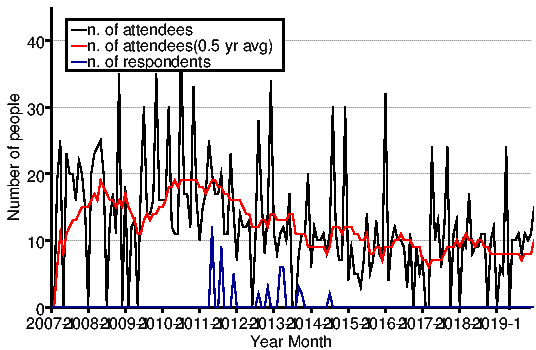
\includegraphics[scale=0.5]{image201912/kansai.png}
	\end{figure}	
\end{frame}

\takahashi[50]{そんな\\こんなで}
\takahashi[120]{次}

\section{事前課題}
\takahashi[50]{事前課題}

\begin{frame}[fragile]
  \frametitle{事前課題}
  \begin{block}{今回の事前課題}
    \begin{enumerate}
    \item Debain デベロッパーリファレンスを読めるようにしておきましょう
    \item \url{https://www.debian.org/doc/manuals/developers-reference/}
    \end{enumerate}
  \end{block}
\end{frame}

\takahashi[50]{Debian パッケージ作成入門2019}

\section{今後の予定}
\begin{frame}[fragile]
  \frametitle{今後の予定}

  \begin{block}{第154回関西Debian勉強会+東海道らぐ+LILO+OpenSUSE}
    \begin{itemize}
    \item 日時: 1月26日(日)
    \item 場所: さくらインターネット、グランドフロント
    \end{itemize}
  \end{block}

\end{frame}

\section{2020 年の予定}
\begin{frame}[fragile]
  \begin{block}{予定}
    \begin{itemize}
        \item 1 月 LT
	\item 2 月以降、wire guard (@znz)  
        \item 3 月?、Rust の package maintainer になりました(Kobayashi)
	\item debian games の辛いこと?  (谷口さん)
	\item CMake で package を作る (otsuki)
	\item 1 月, Mac が購入できたら。Mac でガチの Debian 環境をつくってみた。(佐々木)	
    \end{itemize}
  \end{block}
\end{frame}


\takahashi[50]{}

\end{document}
%%% Local Variables:
%%% mode: japanese-latex
%%% TeX-master: t
%%% End:
